\documentclass[tikz,border=6pt]{standalone}
\usepackage{pgfplots}
\pgfplotsset{compat=1.18}
\usepgfplotslibrary{colormaps}
\usetikzlibrary{arrows, arrows.meta, calc}
\usetikzlibrary{decorations.markings}


\usepackage{amssymb,amsmath,mathtools}

\usepackage[T1]{fontenc}
\usepackage[utf8]{inputenc}
\usepackage{newpxtext,newpxmath}
\usepackage{sectsty}

\newcommand{\Arg}{\textrm{Arg}}

\renewcommand{\Re}{\operatorname{\mathrm{Re}}}
\renewcommand{\Im}{\operatorname{\mathrm{Im}}}

\begin{document}
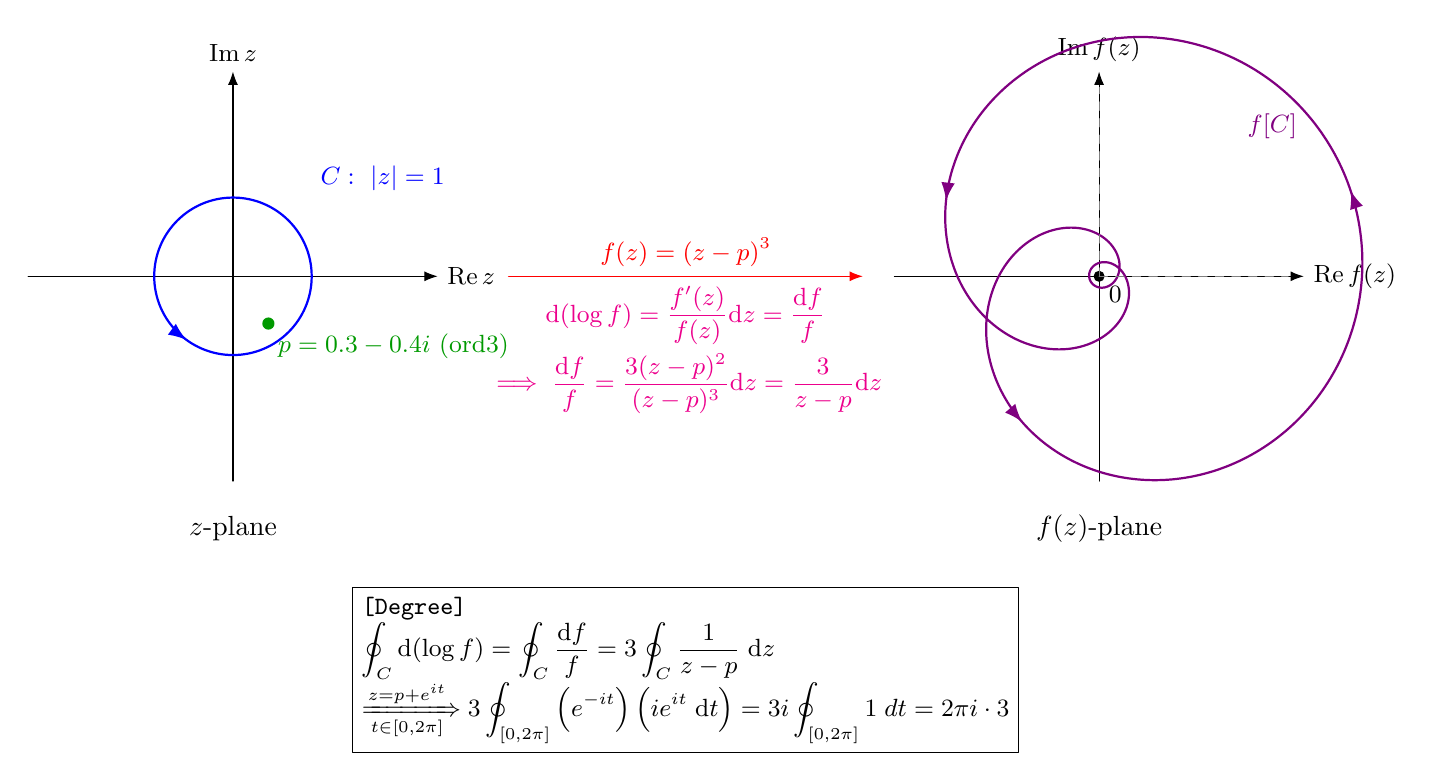
\begin{tikzpicture}[>=Latex, line cap=round, line join=round, font=\small]
%========================
% Left: z-plane
%========================
\begin{scope}[shift={(0,0)}]
\node[font=\normalsize] at (0,-3.2) {$z$-plane};
% axes
\draw[->] (-2.6,0)--(2.6,0) node[right] {$\Re z$};
\draw[->] (0,-2.6)--(0,2.6) node[above] {$\Im z$};

% unit circle C (positively oriented)
\draw[blue,thick,postaction={decorate},
decoration={markings, mark=at position 0.65 with {\arrow{>}}}]
(0,0) circle (1);
\node[blue] at (1.9,1.25) {$C:\ |z|=1$};

% zero at p (order 3), choose concrete p inside C
\fill[green!60!black] (0.45,-0.6) circle(2.2pt) node[below right] {$p=0.3-0.4i$ ($\mathrm{ord} 3$)};
%\node[green!60!black] at (-1.8,1.7) {zero of order $3$};
%\node[red] at (-1.8,-1.7) {poles: none};
\end{scope}

% function label + order via winding form
% annotation: coefficients from Cauchy integral formula at z_0=p
\draw[->, red] (3.5,0) -- (8,0) node[midway, above, align=center] {$\displaystyle
	f(z)=(z-p)^3$};
\draw[->, magenta, opacity=0] (3.5,0) -- (8,0) node[midway, below, align=center, opacity=1] {
	$\displaystyle\mathrm{d}(\log f)=\frac{f'(z)}{f(z)}\mathrm{d}z=\frac{\mathrm{d}f}{f}$\\ [2pt]
	$\displaystyle\implies\frac{\mathrm{d}f}{f}=\frac{3(z-p)^2}{(z-p)^3}\mathrm{d}z=\frac{3}{z-p}\mathrm{d}z$};

\node[draw=black, align=left] at (5.75,-5) {
	\texttt{[Degree]}\\
	$\displaystyle
	\oint_C \mathrm{d}(\log f)=\oint_C \frac{\mathrm{d}f}{f}=3\oint_C \frac{1}{z-p}\; \mathrm{d}z$ \\
	$\displaystyle\xRightarrow[{t\in[0,2\pi]}]{z=p+e^{it}}3\oint_{[0,2\pi]}\left(e^{-it}\right)\left(ie^{it}\; \mathrm{d}t\right)=3i\oint_{[0,2\pi]}1\; dt=2\pi i\cdot 3$
};


%\draw[->] (3.5,0) -- (8,0) node[midway, above, align=center] {$\displaystyle
%f(z)=(z-p)^{3}$};
%\draw[->, opacity=0] (3.5,0) -- (8,0) node[midway, below, align=center, opacity=1] {
%$\displaystyle\oint_C \frac{df}{f}
%=\oint_C \frac{3\,dz}{\,z-p\,}=2\pi i\cdot 3$\\
%$\displaystyle
%a_0=f(p)=\frac{1}{2\pi i}\!\oint_C \frac{f(\zeta)}{\zeta-p}\,d\zeta=0$\\
%$a_1=f'(p)=\frac{1}{2\pi i}\!\oint_C \frac{f(\zeta)}{(\zeta-p)^{2}}\,d\zeta=0,$\\[2pt]
%$\displaystyle
%a_2=\frac{f''(p)}{2!}
%=\frac{1}{2\pi i}\!\oint_C \frac{f(\zeta)}{(\zeta-p)^{3}}\,d\zeta=0$\\
%$a_3=\frac{f^{(3)}(p)}{3!}
%=\frac{1}{2\pi i}\!\oint_C \frac{f(\zeta)}{(\zeta-p)^{4}}\,d\zeta
%=\frac{1}{2\pi i}\!\oint_C \frac{1}{\zeta-p}\,d\zeta=1.$\\[4pt]
%$\mathrm{wind}\big(f(C),0\big)=3
%\ \Rightarrow\
%\displaystyle \oint_C \frac{f'(z)}{f(z)}\,dz=2\pi i\cdot 3.$};

%========================
% Right: f(z)-plane
%========================
\begin{scope}[shift={(11,0)}]
\node[font=\normalsize] at (0,-3.2) {$f(z)$-plane};
% axes
\draw[->] (-2.6,0)--(2.6,0) node[right] {$\Re f(z)$};
\draw[->] (0,-2.6)--(0,2.6) node[above] {$\Im f(z)$};

% origin
\fill (0,0) circle(2pt) node[below right] {$0$};

% image curve f(C): z = 1.5 e^{it} -> w = (z-p)^3
% Let u = 1.5 cos t - 0.3, v = 1.5 sin t + 0.4 (so z-p = u + i v).
% (u+iv)^3 = (u^3 - 3u v^2) + i(3u^2 v - v^3).
\draw[violet,thick,
postaction={decorate},
decoration={markings,
		mark=at position 0.15 with {\arrow{>}},
		mark=at position 0.45 with {\arrow{>}},
		mark=at position 0.75 with {\arrow{>}}}]
plot[domain=0:6.283, samples=650]
({ (1*cos(\x r)-0.3)^(3) - 3*(1*cos(\x r)-0.3)*(1*sin(\x r)+0.4)^(2) },
{ 3*(1*cos(\x r)-0.3)^(2)*(1*sin(\x r)+0.4) - (1*sin(\x r)+0.4)^(3) });
\node[violet] at (2.2,1.9) {$f[C]$};

% dashed rays to visualize winding
\draw[gray,dashed] (0,0) -- (2.4,0);
\draw[gray,dashed] (0,0) -- (0,2.4);
\end{scope}
\end{tikzpicture}	
	
	
	
%\begin{tikzpicture}[>=Latex, line cap=round, line join=round, font=\small]
%
%%========================
%% Left: z-plane
%%========================
%\begin{scope}[shift={(0,0)}]
%	\node[font=\normalsize] at (0,3.2) {$z$-plane};
%	% axes
%	\draw[->] (-2.2,0)--(2.2,0) node[right] {$\Re z$};
%	\draw[->] (0,-2.2)--(0,2.2) node[above] {$\Im z$};
%	
%	% unit circle C (positively oriented) -- radius 1.5 for visibility
%	\draw[blue,thick,postaction={decorate},
%	decoration={markings, mark=at position 0.65 with {\arrow{>}}}]
%	(0,0) circle (1.5);
%	\node[blue] at (1.9,1.0) {$C:\ |z|=1$};
%	
%	% zero at p (order 3), choose concrete p inside C
%	\fill[green!60!black] (0.45,-0.6) circle(2.2pt) node[below right] {$p=0.3-0.4i$};
%	\node[green!60!black] at (-1.8,1.7) {zero of order $3$};
%	\node[red] at (-1.8,-1.7) {poles: none};
%	
%	% function label + order via winding form
%	\node[align=left] at (0,-2.7) {$\displaystyle
%		f(z)=(z-p)^{3},\quad
%		\operatorname{ord}_{p} f
%		=\frac{1}{2\pi i}\!\oint_C \frac{df}{f}
%		=\frac{1}{2\pi i}\!\oint_C \frac{3\,dz}{\,z-p\,}=3.$};
%\end{scope}
%
%%========================
%% Right: w-plane = f(z)-plane
%%========================
%\begin{scope}[shift={(7.2,0)}]
%	\node[font=\normalsize] at (0,3.2) {$w=f(z)$-plane};
%	% axes
%	\draw[->] (-2.8,0)--(2.8,0) node[right] {$\Re w$};
%	\draw[->] (0,-2.8)--(0,2.8) node[above] {$\Im w$};
%	
%	% origin
%	\fill (0,0) circle(2pt) node[below right] {$0$};
%	
%	% image curve f(C): z = 1.5 e^{it} -> w = (z-p)^3
%	% Let u = 1.5 cos t - 0.3, v = 1.5 sin t + 0.4 (so z-p = u + i v).
%	% (u+iv)^3 = (u^3 - 3u v^2) + i(3u^2 v - v^3).
%	\draw[violet,thick,
%	postaction={decorate},
%	decoration={markings,
%		mark=at position 0.15 with {\arrow{>}},
%		mark=at position 0.45 with {\arrow{>}},
%		mark=at position 0.75 with {\arrow{>}}}]
%	plot[domain=0:6.283, samples=650]
%	({ (1.5*cos(\x r)-0.3)^(3) - 3*(1.5*cos(\x r)-0.3)*(1.5*sin(\x r)+0.4)^(2) },
%	{ 3*(1.5*cos(\x r)-0.3)^(2)*(1.5*sin(\x r)+0.4) - (1.5*sin(\x r)+0.4)^(3) });
%	\node[violet] at (2.2,1.9) {$f(C)$};
%	
%	% dashed rays to visualize winding
%	\draw[gray,dashed] (0,0) -- (2.4,0);
%	\draw[gray,dashed] (0,0) -- (0,2.4);
%	
%	% annotation: Taylor coefficients at z_0=p via Cauchy integrals
%	\node[align=center] at (0,-2.55)
%	{$\displaystyle
%		a_0=f(p)=\frac{1}{2\pi i}\!\oint_C \frac{f(\zeta)}{\zeta-p}\,d\zeta=0,\quad
%		a_1=f'(p)=\frac{1}{2\pi i}\!\oint_C \frac{f(\zeta)}{(\zeta-p)^{2}}\,d\zeta=0,$\\[2pt]
%		$\displaystyle
%		a_2=\frac{f''(p)}{2!}
%		=\frac{1}{2\pi i}\!\oint_C \frac{f(\zeta)}{(\zeta-p)^{3}}\,d\zeta=0,\quad
%		a_3=\frac{f^{(3)}(p)}{3!}
%		=\frac{1}{2\pi i}\!\oint_C \frac{f(\zeta)}{(\zeta-p)^{4}}\,d\zeta
%		=\frac{1}{2\pi i}\!\oint_C \frac{1}{\zeta-p}\,d\zeta=1.$\\[4pt]
%		$\mathrm{wind}\big(f(C),0\big)=3
%		\ \Rightarrow\
%		\displaystyle \oint_C \frac{f'(z)}{f(z)}\,dz=2\pi i\cdot 3.$};
%\end{scope}
%
%\end{tikzpicture}
\end{document}